\documentclass[tikz,border=3pt]{standalone}
\usepackage[T1]{fontenc}
\usepackage{mathptmx}
\usepackage{tikz}
\usetikzlibrary{arrows.meta,positioning,calc,fit,shapes.geometric}
\definecolor{forest}{HTML}{346E57}
\definecolor{sage}{HTML}{E8EFEA}
\definecolor{clay}{HTML}{AC653F}
\definecolor{sand}{HTML}{F4EAE2}
\definecolor{ink}{HTML}{252525}
\definecolor{gridgray}{HTML}{D8DAD6}
\tikzset{box/.style={draw=ink!65,line width=.5pt,rectangle,fill=white,align=center,font=\fontsize{10}{11.3}\selectfont,inner sep=5pt}, flow/.style={-{Latex[length=2.1mm]},line width=.65pt,draw=ink!80}, lab/.style={font=\fontsize{10}{11}\selectfont,fill=white,inner sep=2pt,align=center}}
\hyphenpenalty=10000\exhyphenpenalty=10000
\begin{document}
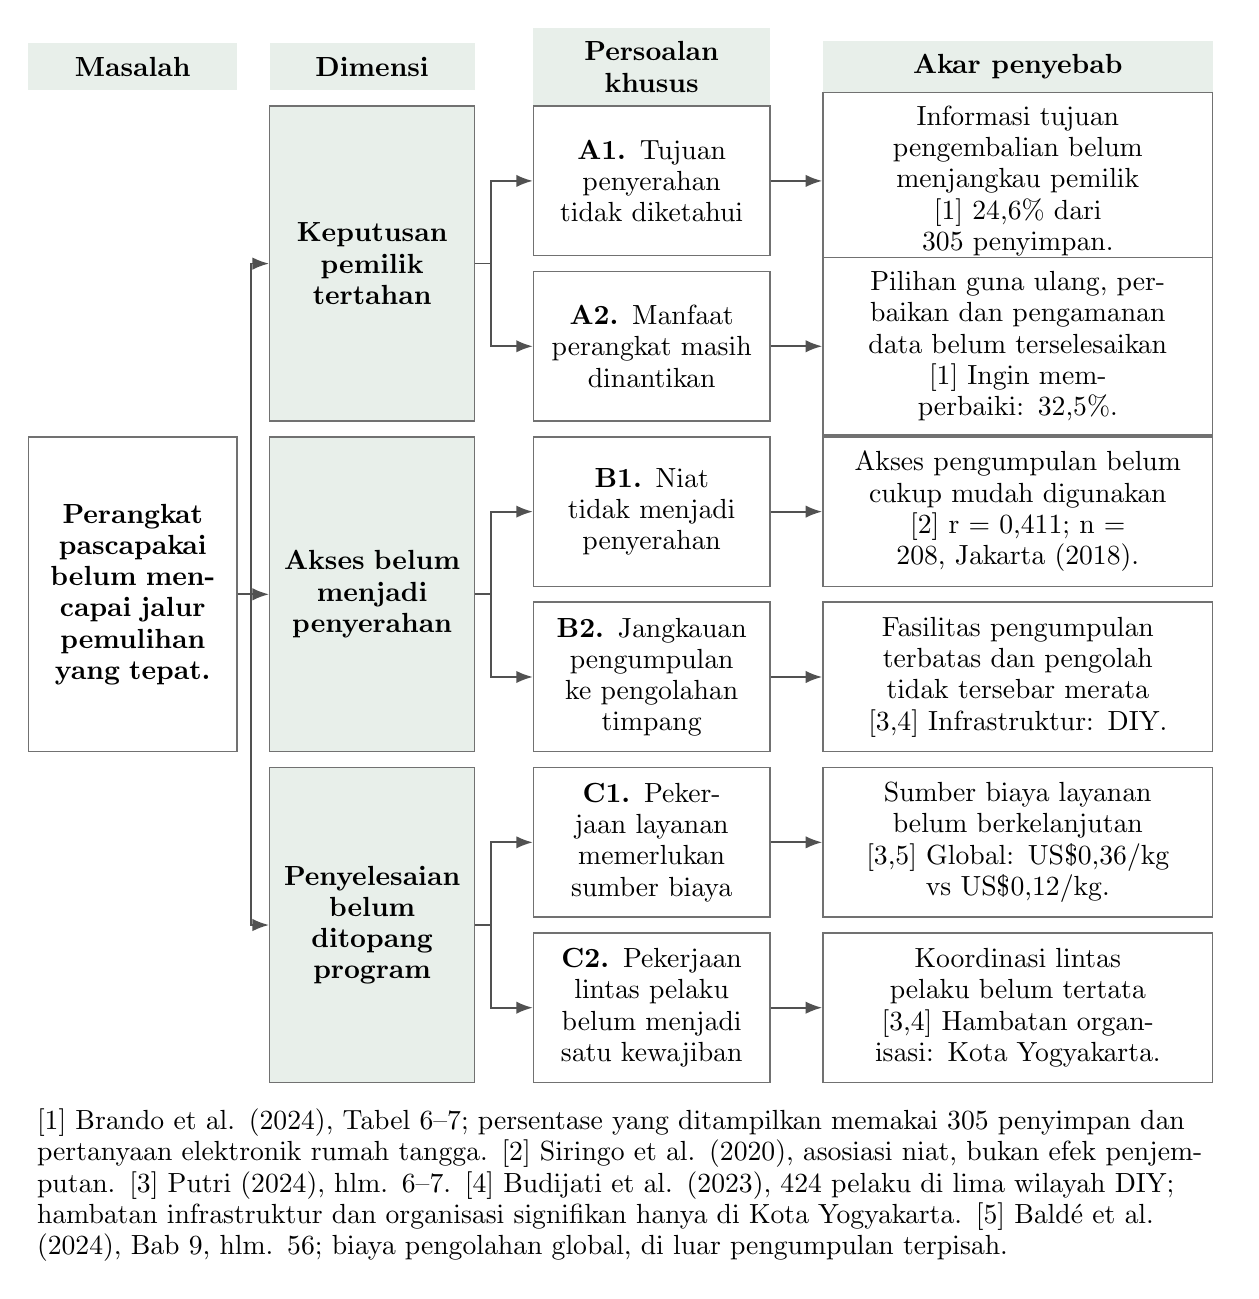
\begin{tikzpicture}[x=1cm,y=1cm]
\node[fill=sage,text width=2.3cm,inner sep=5pt,minimum height=.6cm,align=center,font=\fontsize{10}{11.3}\selectfont\bfseries]at(1.36,11.95){Masalah};
\node[fill=sage,text width=2.25cm,inner sep=5pt,minimum height=.6cm,align=center,font=\fontsize{10}{11.3}\selectfont\bfseries]at(4.4,11.95){Dimensi};
\node[fill=sage,text width=2.65cm,inner sep=5pt,minimum height=.6cm,align=center,font=\fontsize{10}{11.3}\selectfont\bfseries]at(7.95,11.95){Persoalan khusus};
\node[fill=sage,text width=4.6cm,inner sep=5pt,minimum height=.6cm,align=center,font=\fontsize{10}{11.3}\selectfont\bfseries]at(12.6,11.95){Akar penyebab};
\node[box,text width=2.3cm,minimum height=4cm] (problem) at (1.36,5.25){\textbf{Perangkat pascapakai belum mencapai jalur pemulihan yang tepat.}};
\node[box,text width=2.25cm,minimum height=4cm,fill=sage] (dim0)at(4.4,9.45){\textbf{Keputusan pemilik tertahan}};
\draw[flow](problem.east)--++(.17,0)|-(dim0.west);
\node[box,text width=2.65cm,minimum height=1.9cm] (issue0)at(7.95,10.5){\textbf{A1.} Tujuan penyerahan tidak diketahui};
\node[box,text width=4.6cm,minimum height=1.9cm] (cause0)at(12.6,10.5){Informasi tujuan pengembalian belum menjangkau pemilik\\{}[1] 24,6\% dari 305 penyimpan.};
\draw[flow](dim0.east)--++(.2,0)|-(issue0.west);
\draw[flow](issue0.east)--(cause0.west);
\node[box,text width=2.65cm,minimum height=1.9cm] (issue1)at(7.95,8.4){\textbf{A2.} Manfaat perangkat masih dinantikan};
\node[box,text width=4.6cm,minimum height=1.9cm] (cause1)at(12.6,8.4){Pilihan guna ulang, perbaikan dan pengamanan data belum terselesaikan\\{}[1] Ingin memperbaiki: 32,5\%.};
\draw[flow](dim0.east)--++(.2,0)|-(issue1.west);
\draw[flow](issue1.east)--(cause1.west);
\node[box,text width=2.25cm,minimum height=4cm,fill=sage] (dim1)at(4.4,5.25){\textbf{Akses belum menjadi penyerahan}};
\draw[flow](problem.east)--++(.17,0)|-(dim1.west);
\node[box,text width=2.65cm,minimum height=1.9cm] (issue2)at(7.95,6.3){\textbf{B1.} Niat tidak menjadi penyerahan};
\node[box,text width=4.6cm,minimum height=1.9cm] (cause2)at(12.6,6.3){Akses pengumpulan belum cukup mudah digunakan\\{}[2] r = 0,411; n = 208, Jakarta (2018).};
\draw[flow](dim1.east)--++(.2,0)|-(issue2.west);
\draw[flow](issue2.east)--(cause2.west);
\node[box,text width=2.65cm,minimum height=1.9cm] (issue3)at(7.95,4.2){\textbf{B2.} Jangkauan pengumpulan ke pengolahan timpang};
\node[box,text width=4.6cm,minimum height=1.9cm] (cause3)at(12.6,4.2){Fasilitas pengumpulan terbatas dan pengolah tidak tersebar merata\\{}[3,4] Infrastruktur: DIY.};
\draw[flow](dim1.east)--++(.2,0)|-(issue3.west);
\draw[flow](issue3.east)--(cause3.west);
\node[box,text width=2.25cm,minimum height=4cm,fill=sage] (dim2)at(4.4,1.05){\textbf{Penyelesaian belum ditopang program}};
\draw[flow](problem.east)--++(.17,0)|-(dim2.west);
\node[box,text width=2.65cm,minimum height=1.9cm] (issue4)at(7.95,2.1){\textbf{C1.} Pekerjaan layanan memerlukan sumber biaya};
\node[box,text width=4.6cm,minimum height=1.9cm] (cause4)at(12.6,2.1){Sumber biaya layanan belum berkelanjutan\\{}[3,5] Global: US\$0,36/kg vs US\$0,12/kg.};
\draw[flow](dim2.east)--++(.2,0)|-(issue4.west);
\draw[flow](issue4.east)--(cause4.west);
\node[box,text width=2.65cm,minimum height=1.9cm] (issue5)at(7.95,0.0){\textbf{C2.} Pekerjaan lintas pelaku belum menjadi satu kewajiban};
\node[box,text width=4.6cm,minimum height=1.9cm] (cause5)at(12.6,0.0){Koordinasi lintas pelaku belum tertata\\{}[3,4] Hambatan organisasi: Kota Yogyakarta.};
\draw[flow](dim2.east)--++(.2,0)|-(issue5.west);
\draw[flow](issue5.east)--(cause5.west);
\node[anchor=north west,text width=15.05cm,align=left,font=\fontsize{10}{11.3}\selectfont]at(.02,-1.16){[1] Brando et al. (2024), Tabel 6–7; persentase yang ditampilkan memakai 305 penyimpan dan pertanyaan elektronik rumah tangga. [2] Siringo et al. (2020), asosiasi niat, bukan efek penjemputan. [3] Putri (2024), hlm. 6–7. [4] Budijati et al. (2023), 424 pelaku di lima wilayah DIY; hambatan infrastruktur dan organisasi signifikan hanya di Kota Yogyakarta. [5] Baldé et al. (2024), Bab 9, hlm. 56; biaya pengolahan global, di luar pengumpulan terpisah.};
\end{tikzpicture}
\end{document}
